%Assignment 2 
%Vikas Kurapati
%130010058
\documentclass[11pt, a4paper]{article}
\usepackage[affil-it]{authblk} 
\usepackage{etoolbox}
\usepackage{lmodern}
\usepackage{titlesec}
\usepackage{float}

\makeatletter
\patchcmd{\@maketitle}{\LARGE \@title}{\fontsize{20}{19.2}\selectfont\@title}{}{}
\makeatother

\renewcommand\Authfont{\fontsize{16}{14.4}\selectfont}
\renewcommand\Affilfont{\fontsize{12}{10.8}\itshape}

\title{\textbf{Assignment 2}} 
\author{Vikas Kurapati - 130010058}
\usepackage{graphicx}
\begin{document}
\maketitle
\newpage
\section{Question1:}
\subsection{ODE for Normalized Sheath Potential}
The normalized sheath potential $V = \frac{e(\phi_{se} - \phi)}{k T_e}$ with normalized distance $\eta = \frac{x - x_{se}}{\lambda_D}$ for $M_{se} = 1$ is given by
\begin{equation}
 \frac{d^2 V}{d\eta^2} = \frac{1}{\sqrt{1 + 2V}} - e^{-V}
\end{equation}

\subsection{Expression for normalized sheath electric field \textbf{$\frac{dV}{d\eta}$}}
Expression for normalized sheath electric field $\frac{dV}{d\eta}$ for $\frac{dV}{d\eta} = \epsilon$ at $\eta = 0$ is given by
\begin{equation}
 \frac{dV}{d\eta} = \sqrt{\epsilon^2 + 2(\sqrt{1 + 2V} + e^{-v} -2)}
\end{equation}

\section{Question 2}
\subsection{Bohm Condition}
The form it takes in the Bohm $(V\ll1)$ case is:
\begin{equation}
 \frac{dV}{d\eta} = \epsilon \Rightarrow V(\eta) = \epsilon \eta
\end{equation}

where $\epsilon$ is $\frac{dV}{d\eta}$ at $\eta = 0$

\subsection{Child-Langmuir Limits}
The form it takes in the Child-Langmuir $(V\gg1)$ case is:
\begin{equation}
 V(\eta) = \frac{3^{\frac{4}{3}}}{2^\frac{5}{3}} \eta^{\frac{4}{3}} \Rightarrow \frac{dV}{d\eta} = 6^\frac{1}{3} \eta^\frac{1}{3}
\end{equation}

\section{Question 3}
\subsection{Normalized electric Field}
Plots comparing the RHS for normalized electric field for the three cases:
\begin{figure}[H]
 \centering
 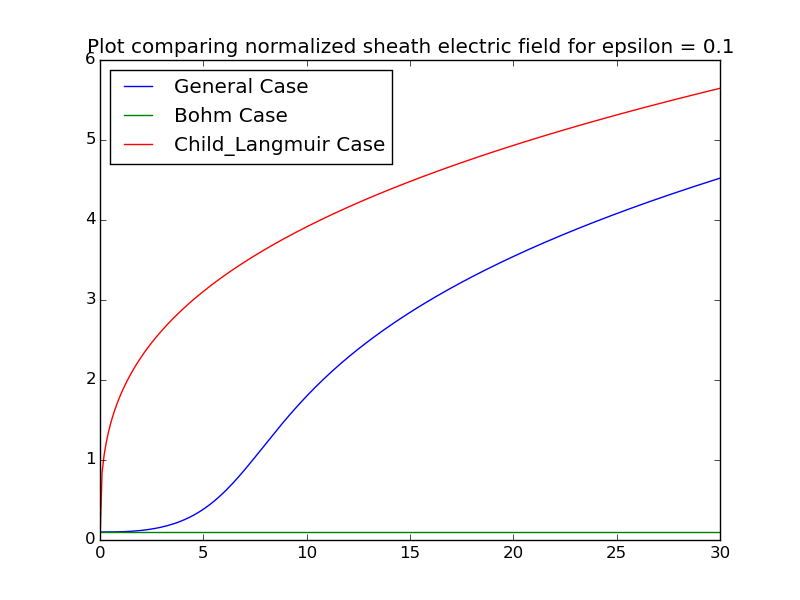
\includegraphics[width = \textwidth]{q3Eeps1.png}
\end{figure}
\begin{figure}[H]
 \centering
 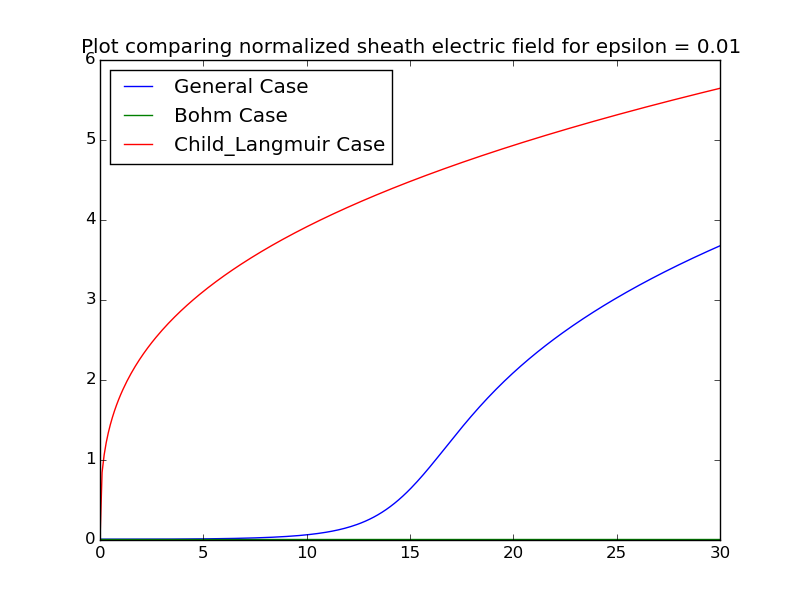
\includegraphics[width = \textwidth]{q3Eeps2.png}
\end{figure}

\begin{figure}[H]
 \centering
 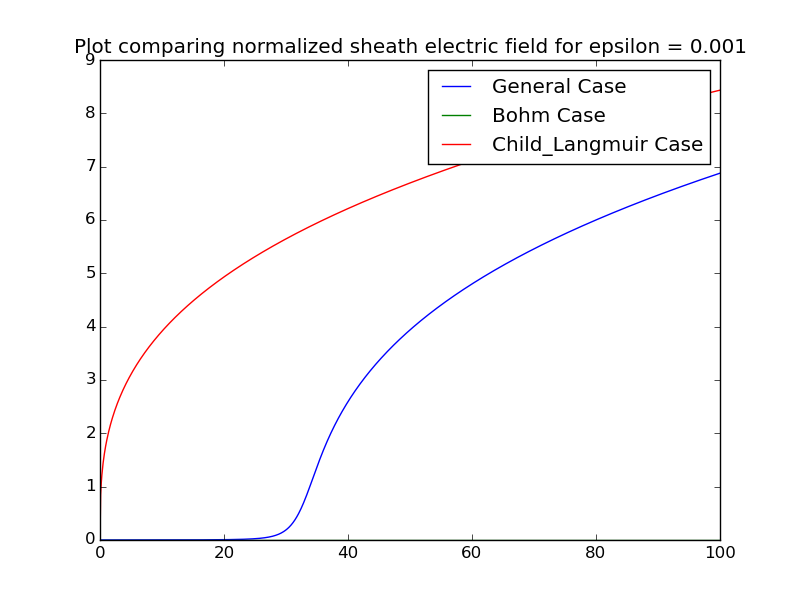
\includegraphics[width = \textwidth]{q3Eeps3.png}
\end{figure}

\subsection{Normalized Potential}
Plots comparing the RHS for normalized Potential for the three cases:
\begin{figure}[H]
 \centering
 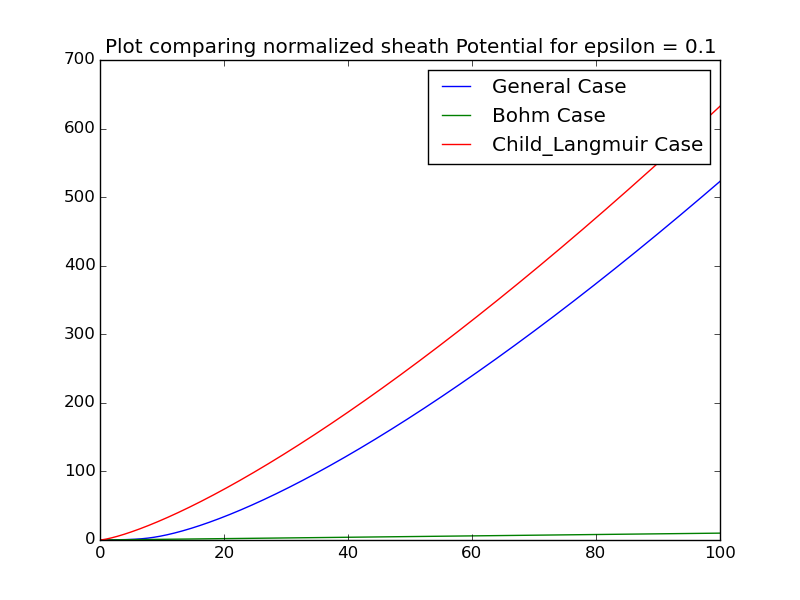
\includegraphics[width = \textwidth]{q3Veps1.png}
\end{figure}
\begin{figure}[H]
 \centering
 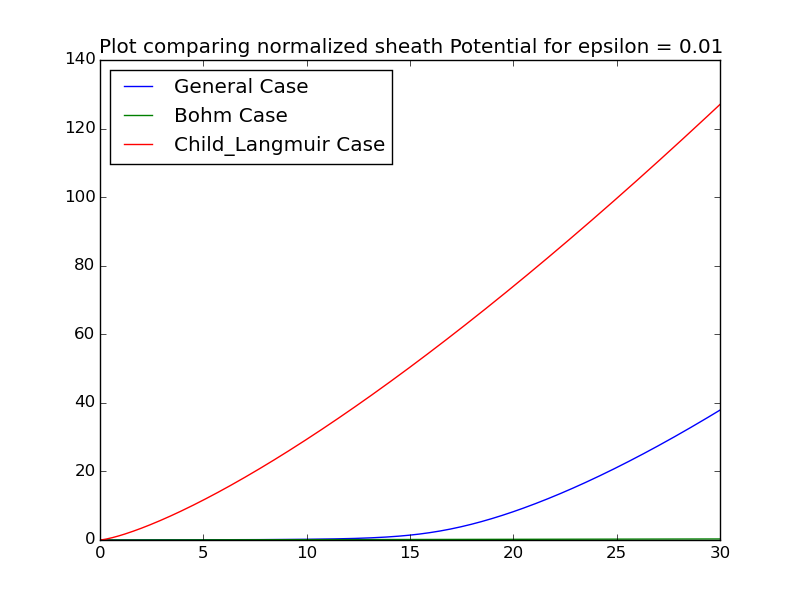
\includegraphics[width = \textwidth]{q3Veps2.png}
\end{figure}

\begin{figure}[H]
 \centering
 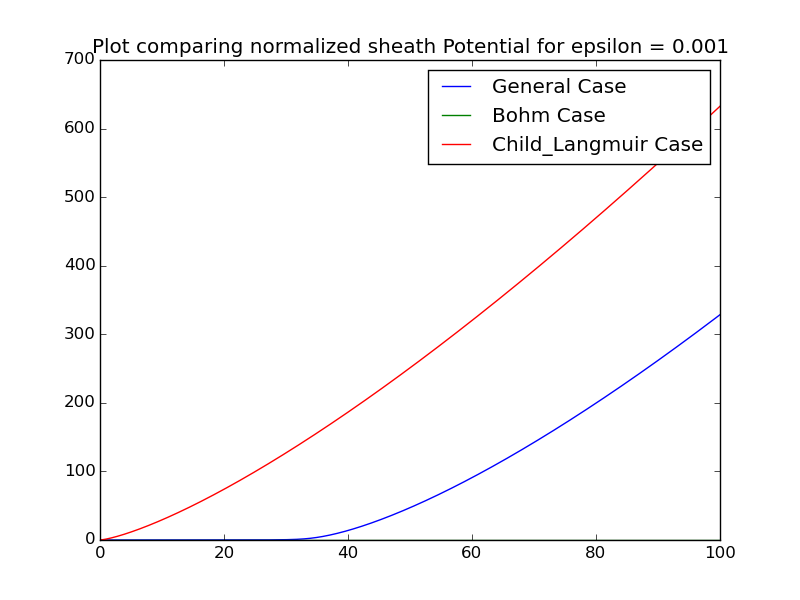
\includegraphics[width = \textwidth]{q3Veps3.png}
\end{figure}

\section{Question 4}
The exact solution derived for wall potential is $V_w = \frac{1}{2}ln(\frac{m_i}{2\pi m_e}) \approx 2.83$ 
(Refer Code)
\begin{itemize}
 \item Sheath thickness normalized with debye length to reach wall potential for $\epsilon = 0.100000$ is 7.815631
 \item Sheath thickness normalized with debye length to reach wall potential for $\epsilon = 0.010000$ is 16.633267
 \item Sheath thickness normalized with debye length to reach wall potential for $\epsilon = 0.001000$ is 34.368737
 \item Sheath thickness normalized with debye length to reach wall potential for $\epsilon = 0.000100$ is 71.671672
  \item Sheath thickness normalized with debye length to reach wall potential for $\epsilon = 0.000010$ is 151.615162
  \item Sheath thickness normalized with debye length to reach wall potential for $\epsilon = 0.000001$ is 323.832383
\end{itemize}

\section{Question 5}
The normalized electric field is given for different cases of $\epsilon$ are 
\begin{itemize}
 \item The normalized electric field for $\epsilon = 0.100000$ is 1.140026
  \item normalized electric field for $\epsilon = 0.010000$ is 1.135212
  \item The normalized electric field for $\epsilon = 0.001000$ is 1.159439
  \item The normalized electric field for $\epsilon = 0.000100$ is 1.154175
  \item The normalized electric field for $\epsilon = 0.000010$ is 1.146671
  \item The normalized electric field for $\epsilon = 0.000001$ is 1.159135
\end{itemize}

\section{Question 6}
(Refer Code)
\begin{itemize}
 \item Child Langmuir starts at eta = 0.080000 for epsilon = 0.010000 for V = 1.000000
  \item The thickness of sheath for a neutral wall with epsilon = 0.100000 and electrode potential = 1.000000 is 0.140000
  \item Child Langmuir starts at eta = 0.080000 for epsilon = 0.010000 for V = 10.000000
  \item The thickness of sheath for a neutral wall with epsilon = 0.100000 and electrode potential = 1.000000 is 0.170000
  \item Child Langmuir starts at eta = 0.080000 for epsilon = 0.010000 for V = 100.000000
  \item The thickness of sheath for a neutral wall with epsilon = 0.100000 and electrode potential = 1.000000 is 0.210000
  \item Child Langmuir starts at eta = 0.080000 for epsilon = 0.010000 for V = 1.000000
  \item The thickness of sheath for a neutral wall with epsilon = 0.010000 and electrode potential = 1.000000 is 0.140000
  \item Child Langmuir starts at eta = 0.080000 for epsilon = 0.010000 for V = 10.000000
  \item The thickness of sheath for a neutral wall with epsilon = 0.010000 and electrode potential = 1.000000 is 0.170000
  \item Child Langmuir starts at eta = 0.080000 for epsilon = 0.010000 for V = 100.000000
  \item The thickness of sheath for a neutral wall with epsilon = 0.010000 and electrode potential = 1.000000 is 0.210000
  \item Child Langmuir starts at eta = 0.120000 for epsilon = 0.001000 for V = 1.000000
  \item The thickness of sheath for a neutral wall with epsilon = 0.010000 and electrode potential = 1.000000 is 0.170000
  \item Child Langmuir starts at eta = 0.120000 for epsilon = 0.001000 for V = 10.000000
  \item The thickness of sheath for a neutral wall with epsilon = 0.010000 and electrode potential = 1.000000 is 0.210000
  \item Child Langmuir starts at eta = 0.120000 for epsilon = 0.001000 for V = 100.000000
  \item The thickness of sheath for a neutral wall with epsilon = 0.010000 and electrode potential = 1.000000 is 0.240000

\end{itemize}

\end{document}